\documentclass[12pt]{article}
\setlength{\textwidth}{17cm}
\setlength{\textheight}{24cm}
\setlength{\topmargin}{-2cm}
\setlength{\footskip}{1cm}
\setlength{\evensidemargin}{0cm}
\setlength{\oddsidemargin}{0cm}
\setlength{\parindent}{0cm}

\usepackage{allrunes}
\usepackage{amsmath}
\usepackage[magyar]{babel}
\usepackage[T1]{fontenc}
\usepackage[utf8]{inputenc}
\usepackage{fixltx2e}
\usepackage{multirow}

\usepackage[hyphens]{url}
\usepackage[unicode,colorlinks=true,breaklinks]{hyperref}
%\usepackage[dvips]{hyperref}
%should display links, but it does not work with \H accent
%and formulas in section titles

\hypersetup{colorlinks,linkcolor=blue,urlcolor=magenta,citecolor=magenta}
%Breaks long url`s in text, while keeping it one link:

\usepackage{amsfonts}
\usepackage{amsthm}
\usepackage{amssymb}


\theoremstyle{plain}
\usepackage{graphicx}

%\usepackage{gensymb}
\usepackage{float}

% For bra-ket notation
\usepackage{braket}

%% New commands
\newcommand{\dd}{\textrm{d}}

%% Pauli matrices
\newcommand{\sigx}{\sigma_x}
\newcommand{\sigy}{\sigma_y}
\newcommand{\sigz}{\sigma_z}

\newcommand{\paulix}{
    \left( \begin{array}{cc}
        0 & 1 \\
        1 & 0
    \end{array}
    \right)
}

\newcommand{\pauliy}{
    \left( \begin{array}{cc}
        0 & -i \\
        i & 0
    \end{array}
    \right)
}

\newcommand{\pauliz}{
    \left( \begin{array}{cc}
        1 & 0 \\
        0 & -1
    \end{array}
    \right)
}

% \begin{figure}[H]
%     \begin{center}
%     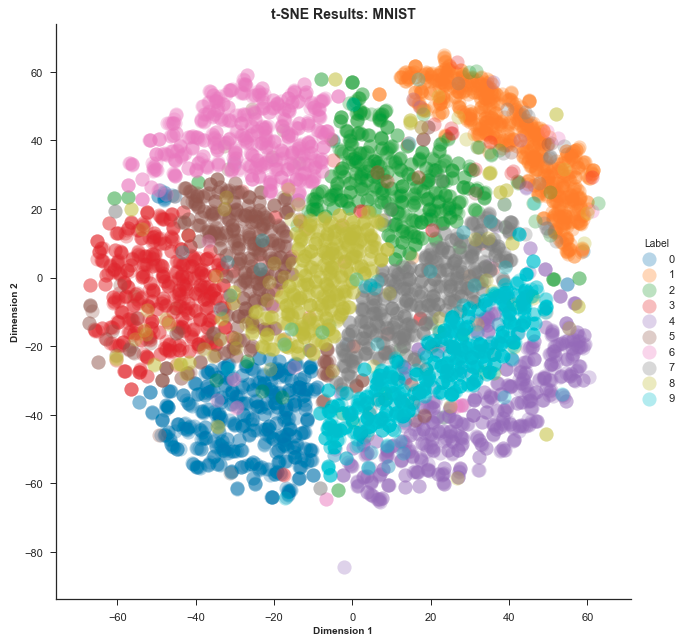
\includegraphics[width=0.5\textwidth]{media/tsneplot.png}
%     \caption{t-SNE plot for MNIST dataset \cite{tsne-article}} 
%     \label{fig:tsneplot}
%     \end{center}
% \end{figure}

\begin{document}
\title{\textbf{1. tétel}}
\author{Berekméri Evelin}

\maketitle


\newpage
\begin{abstract}
    Mérési adatok és a mérési hiba – Hibák és zajok, ezek forrásai. A statisztikus és a szisztematikus hiba. A hiba sztochasztikus modellezése. Adatmodellezés – A függvényillesztés alapproblémája. Magfüggvényes becslések.
\end{abstract}

\section*{Mérési adatok és a mérési hiba – Hibák és zajok, ezek forrásai.}
A mérés célja a mérendő mennyiség valódi értékének meghatározása. A méréseket műszerrel végezzük, amiknek van mérési tartománya és mérési pontossága. Ha a műszer nem elég érzékeny, a mért érték egy felső korlát, ha a műszer túl érzékeny a mért érték egy alsó korlát. A mért adatok hibával terheltek, a valódi értéket csak közelíteni tudjuk a mérési adatok segítségével.  A mért mennyiséget hibával együtt kell közölni. Mérési hibák típusai:
\begin{itemize}
    \item leolvasási hiba: a műszer felbontásából ered, az utolsó értékes számjegy fele (pl. centis beosztású mérőeszköz esetén 0.5 cm)
    \item statisztikus hiba
    \item szisztematikus hiba
    \item (zaj: külső környezetből származó, a fizikai folyamat jellegéből származó)
\end{itemize}

\section*{Statisztikus hiba}
A statisztikus hibák nem ismert vagy nem ellenőrizhető tényezők következményei, hatásuk kicsi, egymástól független, mérésenként változó, véletlenszerű. Ilyen tényező lehet például: külső mechanikus, elektronikus, mágneses zaj, légmozgás, hőmérsékletingadozás vagy okozhatja a műszer véletlenszerű működése. A mérendő mennyiség is lehet statisztikus jellegű: pl. a rúd átmérője ingadozik a hossza mentén, az időegység alatt elbomlott atomok száma. A statisztikus hibák esetén a mérés többszöri megismétlésével a mérendő mennyiség valódi értékét egyre jobban közelítjük az átlaggal: $\overline{y} = \frac{\sum_{i=1}^{n} y_i}{n}$, ahol $y_i$ különböző mérési eredmények. Ezt az átlagot nevezik empirikus várható értéknek is.  Ha a mérési hiba sok független valószínűségi változó átlagaként áll
elő, akkor érvényes rá a centrális határeloszlás tétel, azaz a hiba eloszlása Gauss-eloszlást követ és a hiba nagyságát a Gauss-eloszlás szórása jellemzi. A statisztikus hibát továbbá lehet csökkenteni a külső tényezők hatásának csökkentésével, pl hűtjük a műszert vagy elektromágnesesen árnyékoljuk.






\section*{Szisztematikus hiba}
A szisztematikus hibák a mérések többszöri megismétlésével hasonló mértékben jelentkeznek, nem véletlenszerűek, nem küszöbölhetők ki statisztikus módszerekkel. Lehet állandó (nullponti hiba) és függhet a mért értéktől is.  Eredhetnek: 
\begin{itemize}
    \item a mérőeszköz pontatlanságából: pl. mérőeszköz rossz kalibrációja vagy pl ha a mérőrúd hossza 1 m helyett 99,9 cm, a mért értékék mindig eltérnek egy állandó értékkel a pontosabb rúddal mért értéktől
    \item a mérési módszerből: pl. ha a mágneses tér mérésekor egy ismeretlen külső forrásból eredő tér adódik hozzá a mérési eredményekhez. A szisztematikus hiba csökkenthető ebben az esetben, ha a mérést több módszerrel vagy másik laboratóriumban végezzük el.
    \item a mérés során ismeretlen körülmény is okozhatja.
\end{itemize}
A szisztematikus hibák felderítéséhez:
\begin{itemize}
    \item a mérőberendezést kalibráljuk: egy hitelesített mérőeszközzel hasonlítjuk össze
    \item a mérőeszköz gyártója is megadhatja a mért értékre vonatkozóan hány százalék a hiba
\end{itemize}
Újabb mennyiség származtatása esetén közelítő képletet csak akkor használjuk, ha az így kapott hiba nem nagyobb az egyéb hibáknál, különben használjuk pontosabb képletet.


\section*{A hiba sztochasztikus modellezése}
\textit{A sztochasztikus hibáról akkor beszélünk, amikor annak ellenére, hogy jó a modell és a paraméterek, a várható eredménytől különbözőt kapunk. Ez szimulációval becsülhető vagy eloszlásokból számolható. 
}

\section*{Adatmodellezés – A függvényillesztés alapproblémája}
%Adatmodellezéskor választunk egy elméletileg megfelelő függvényalakot és a függvény paramétereit úgy állítjuk be, hogy az valamilyen szempont szerint a lehető legjobban illeszkedjen a mért adatokra. 

Adatmodellezéskor az elméleti modell bizonyos $x_i$ változók és a paraméterek függvényében becslést ad a mérhető fizikai mennyiségek értékeire. A modell lehet:
\begin{itemize}
    \item matematikai: függvényillesztés (ilyenkor az $x_i$ értékek adottak. választunk egy elméletileg megfelelő függvényalakot és a függvény paramétereit úgy állítjuk be, hogy a modell által adott $y(x_i
|a)$ becslések valamilyen szempont szerint a lehető legjobban illeszkedjenek az $y_i$ mért értékekre. $y(x_i
|a) = f(x_i, a)$ )
    \item szimulációs: numerikus algoritmus
\end{itemize}
Ha a modell szerint a mérési eredmények egymástól függetlenek, és kizárólag az $x_i$ értékektől és az ismeretlen a paraméterektől függnek, akkor használhatjuk a maximum likelihood módszerét (2.tétel). 


Egy adott mért érték valamilyen $P(y_i)$ valószínűséggel fordul elő. A $P(yi)$ valószínűség eloszlása megismételt mérésekkel megbecsülhető, standard hiba esetében ez normális eloszlás, a mérési hibának
megfelelő $\sigma$ szórással (a modell része az is, hogy a hiba milyen eloszlású). 

Függvényillesztésnél gyakran érdemes megszabadulni a kilógó pontoktól (outlierektől), amik $3 \sigma$-n kívűl esnek. 

\subsection*{Legkisebb négyzetek módszere}
A legkisebb négyezetek módszerét a mért mennyiségek közötti függvénykapcsolat analitikus alakjának meghatározásához használjuk. Van n db ($x_i, y_i$) mérési pontunk. Az x, y mért mennyiségek között lineáris kapcsolatot feltételezünk:
$$ y = mx+b. $$ A mérés célja az m meredekség és b tengelymetszet meghatározása és a lineáris kapcsolat igazolása. A legkisebb négyzetek módszere főképp akkor alkalmazható, ha csak az y értékek rendelkeznek statisztikus hibával és az $y_i$ értékek szórása minden $x_i$ pontban azonos és az x értékeknek nincs hibája. Ez a gyakorlatban általában azt jelenti, hogy az x értékeket pontosabban tudjuk mérni. 

Keressük azt az $$ y = \hat{m}x+\hat{b} $$ egyenest, amely a legjobban illeszkedik a mért n db pontra, $\hat{m}$ és $\hat{b}$ a valódi egyenes m és b paramétereinek becslései a mérési pontok alapján, mivel az ($x_i, y_i$) mért értékpárok hibával rendelkeznek.  Az $x_i$ pontban az egyenes az $$ y_i* = \hat{m}x_i+\hat{b} $$ értéket veszi fel. Az eltérés a mért pontok és az egyenes pontjai között $$ y_i -y_i* = y_i - (\hat{m}x+\hat{b}). $$ Akkor illeszkedik a legjobban az egyenesen a pontokra, ha az eltérések négyzetösszege minimális, tehát keressük $$ S(\hat{m}, \hat{b}) = \sum_{i=1}^n (y_i - (\hat{m}x+\hat{b}) )^2 $$ minimumát $\hat{m}$ és $\hat{b}$ függvényében: $$ \frac{\partial S(\hat{m}, \hat{b})}{\partial \hat{m}} = 0, \frac{\partial S(\hat{m}, \hat{b})}{\partial \hat{b}} = 0. $$ Innen $\hat{m}, \hat{b}$ kiszámolható. Részletesen levezetés: \cite{klasszfiz}. Az így kapott paraméterekkel megrajzolt egyenes regressziós egyenes, az eljárás neve pedig lineáris regresszió.  A legkisebb négyzetek módszere a maximum likelihood speciális esete, amikor $\sigma $ konstans, normális eloszlású és kiemelhető a $\chi^2$-ből. Ez részletesebben: 2.tétel vagy \cite{dobos}. 

A legkisebb négyzetek módszere akkor is alkalmazható, ha a kapcsolat az x és y értékek között nem lineáris. Ilyenkor többnyire nem lineáris egyenletrendszerekkel megoldásával keressük a paramétereket. De van lehetőség bizonyos összefüggéseket lineárissá alakítani, például logaritmussá alakítással. Pl. $y = a e ^ {bx} \rightarrow \ln y = \ln a + bx$.  

Az illesztés \ lineáris regresszió jóságát jellemzi a  korrelációs együttható:
$$ r = \frac{\sigma_{i=1}^n (x_i - \overline{x}) (y_i - \overline{y})}{\sqrt{ \sigma_{i=1}^n (x_i - \overline{x})^2 \sigma_{i=1}^n (y_i - \overline{y})^2}}. 
$$ $|r| \leq 1 $ és r előjele megegyezik az illesztett egyenes meredekségével. Ha minden pont az egyenesen van $|r| = 1 $. 

\section*{Magfüggvényes becslések (kernel smoothing)}
Diszkrét  mintavételezéssel történő megfigyeléssel önmagában nem jellemezhetjük jól a folytonosan leírható jelenségeket. 

A $K:R \rightarrow [0, \infty]$  függvényt magfüggvénynek nevezzük, ha K korlátos, folytonos, szimmetrikus sűrűségfüggény, melyre teljesülnek a következő feltételek: 
$$ lim_{|x| \rightarrow \infty} |x| K(x) = 0, \int_{-\infty}^{\infty}  x^2 K(x) dx < \infty. $$

Adott egy f(x) függvény, melyből az [a,b] intervallumon veszünk n db mintát ($X_i$). Legyen $h_n$ pozitív egész szám, melyet sávszélességnek nevezünk. A magfüggvény becslés alakja a következő: 

$$
\hat{f_n}(x) = (n h_n)^{-1} \sum_{i=1}^n K(\frac{x-X_i}{h_n}) = n^{-1} \sum_{i=1}^n K_h(x-X_i),
$$ ahol $K_h(u) = h_n^{-1}K(u/h_n)$. 

A magfüggvény becslés technika alkalmazható: 
\begin{itemize}
    \item az elméleti összefüggést leíró folytonos függvény becslésésére véges, diszkrét mintapontokból
    \item adat simításra, a mintavételezési eljárás során fellépő hibák csillapítására, a mérési folyamat során átszűrődő zaj kiszűrésére
    \item neurális hálózatok betanítási fázisában. 
\end{itemize}



%\bibliographystyle{plain}
%\bibliography{references}

\begin{thebibliography}

\bibitem{dobos}
\url{http://www.vo.elte.hu/~dobos/teaching/fiznum2019/slides/02.pdf}, \url{http://www.vo.elte.hu/~dobos/teaching/fiznum2019/slides/01.pdf}

\bibitem{klasszfiz}
\url{http://metal.elte.hu/oktatas/klaszfizlab/klasszikus_labor_anyaga.pdf}

\end{thebibliography}

\end{document}